

%%%%%%%%%%%%%%%%%%%%%%%% ADD CONTENT %%%%%%%%%%%%%%%%%%%%%%
\section{Work Structure /& Version Control}
% specific header SJ slides
% pengu with E for example, T task, ! take home message
%=============================================================================================
 
\begin{frame}{\insertsectionnumber{ |} Reality Check}
\begin{columns}
\column[c]{5cm}

\begin{beamerboxesrounded}[lower=gray,shadow=true]{
I plotted this real nice figure for Richard a while ago.  Now Peter wants something very similar. The graph just needs a different colormap. Wish I used a damn script and saved it.
}
\end{beamerboxesrounded}
% work with scripts and save them with your figure
\vspace*{0.2cm}
\begin{beamerboxesrounded}[lower=gray,shadow=true]{
I wrote this really flash paragraph about extra-terrestian fossils in my samples. Rob thought it was bogus.  Now that they have landed in Area 51 to collect their trash I would really like that paragraph back in the maunscript. 
}
\end{beamerboxesrounded}
% version control, backup
\vspace{0.3cm}

\column[c]{5cm}

%\begin{beamerboxesrounded}[lower=gray,shadow=true]{
%I just discovered a really cool feature in one of the 50+ simulations from last year. \\
%What was the vertical diffusion I used in that simulation? And how warm was the atmospheric forcing data?
%}
%\end{beamerboxesrounded}
% naming convention, backup

% instant backup

\vspace{0.2cm} \hspace{1cm}

\includegraphics[height=3cm]{./images/bucket.jpg}
%\end{itemize}
\end{columns}
\end{frame}

%=============================================================================================
 
\begin{frame}{\insertsectionnumber{ |} Reality Check}
\begin{columns}
\column[c]{5cm}

\begin{beamerboxesrounded}[lower=gray,shadow=true]{
I plotted this real nice figure for Richard a while ago.  Now Peter wants something very similar. The graph just needs a different colormap. Wish I used a damn script and saved it.
}
\end{beamerboxesrounded}
% work with scripts and save them with your figure
\vspace*{0.2cm}
\begin{beamerboxesrounded}[lower=gray,shadow=true]{
I wrote this really flash paragraph about extra-terrestian fossils in my samples. Rob thought it was bogus.  Now that they have landed in Area 51 to collect their trash I would really like that paragraph back in the maunscript. 
}
\end{beamerboxesrounded}
% version control, backup
\vspace{0.3cm}
\textbf{
\begin{itemize}
\item How do you work?
\item What is your workflow?
\item Does your work structure map your workflow?
\end{itemize}
}
\column[c]{5cm}

%\begin{beamerboxesrounded}[lower=gray,shadow=true]{
%I just discovered a really cool feature in one of the 50+ simulations from last year. \\
%What was the vertical diffusion I used in that simulation? And how warm was the atmospheric forcing data?
%}
%\end{beamerboxesrounded}
% naming convention, backup

\begin{beamerboxesrounded}[lower=gray,shadow=true]{
Finally got around to publish some of that ancient thesis material from 5 years ago.  Just got an email from the journal's editor, requesting a re-plot of figures in high res.
}
\end{beamerboxesrounded}
\vspace*{0.2cm}
\begin{beamerboxesrounded}[lower=gray,shadow=true]{
Lockdown was fun - got lots of processing and writing done. Will copy and backup files when I get back to the office next week. \\
... \\
My labtop dropped off the table last night. The hard drive is jammed.
}
\end{beamerboxesrounded}
% instant backup

\vspace{0.2cm} \hspace{1cm}

\includegraphics[height=3.0cm]{./images/fishbones.jpg} \hspace{-0.2cm} 
\includegraphics[height=0.8cm]{./images/brokencomputer.jpg}
%\end{itemize}
\end{columns}
\end{frame}

%=============================================================================================
%
%\begin{frame}{\insertsectionnumber{ |} Reality Check}
%\begin{columns}
%\column[c]{5cm}
%% 
%\begin{beamerboxesrounded}[lower=gray,shadow=true]{
%Plotting Scripts \\
%  
%Naming  \\
%  
%Backup \\
%  
%}
%\end{beamerboxesrounded}
%%% work with scripts and save them with your figure
%\vspace*{0.2cm}
%
%\begin{beamerboxesrounded}[lower=gray,shadow=true]{
%
%
%Version Control \\
%
%
%Backup \\
%
%
%}
%\end{beamerboxesrounded}
%%% version control, backup
%
%\column[c]{5cm}
%%
%\begin{beamerboxesrounded}[lower=gray,shadow=true]{
%Naming \\
%
%
%Data Handling \\
%
%
%Folder Structure \\
%}
%\end{beamerboxesrounded}
%%% naming convention, backup
%%
%\vspace*{0.2cm}
%\begin{beamerboxesrounded}[lower=gray,shadow=true]{
%Instant Backup \\
%Cross Desk syncronization
%}
%\end{beamerboxesrounded}
%%% instant backup
%%
%\vspace*{0.2cm}
%\begin{beamerboxesrounded}[lower=gray,shadow=true]{
%Backup \\
%
%Naming \\
%
%Version Control \\
%
%
%Plotting Scrits \\
%
%ARchiving \\
%}
%\end{beamerboxesrounded}
%%
%%
%\end{columns}
%\begin{itemize}
%\item How do you work?
%\end{itemize}
%\end{frame}

%=============================================================================================
%
\begin{frame}{\insertsectionnumber{ |} Workflow}

%\item \textbf{What is a workflow?} \\
%Wikipedia \\
\textit{"A workflow consists of an orchestrated and \textbf{repeatable} pattern of activity, enabled by the systematic organization of resources into processes that transform matericals, provide services, or process information."} (Wikipedia)
\begin{itemize}
\item Examples 
\begin{itemize}
\item[\textbullet] All physical and mental steps between your hypothesis and the published result. \\
\item[\textbullet] All related tasks and stages to carry out an experiment. \\
\item[\textbullet]All activities, materials and documents to measure a rock sample.
\end{itemize}

\end{itemize}

\begin{columns}

\column[c]{7.5cm}

\begin{itemize}

\item \textbf{Why do we need to think about our workflows?}

\item Repeatability and reproducability are key requirements in science. For example \\
\begin{itemize}

\item[\textbullet] Result of a numerical model. \\
\item[\textbullet] Chemical analysis of a rock sample. \\
\item[\textbullet] Pre-processing of a dataset. \\
\item[\textbullet] A figure in a publication. 
\end{itemize}
\item Maximizes work efficiency and increases effectiveness. 
\end{itemize}

\column[c]{2cm}

\includegraphics[height=3cm]{./images/walkman.jpg}

\end{columns}

\end{frame}

%=============================================================================================
\begin{frame}{\insertsectionnumber{ |} Workflow - concept \&  terminology}

\hspace{2cm}
\begin{beamerboxesrounded}[lower=gray,shadow=true]{
\begin{columns}

\column[c]{2.5cm}
\footnotesize{
\textbf{State} \\
Product \\
Result \\
Milestone \\
Information \\
Resource 
}

\column[c]{2.5cm}
\footnotesize{
File \\
Figure \\
data set \\
Sample \\
Accepted publication \\
document 
}
\end{columns}
}
\end{beamerboxesrounded}

\begin{columns}
\column[c]{3cm}
\begin{beamerboxesrounded}[lower=gray,shadow=true]{
\footnotesize{
\textbf{Process} \\
Activity \\
Conversion \\
transformation \\
Transition \\
\\
\textbf{Examples} \\
Writing \\
Dissolving a rock sample \\
Cropping a data set \\
Plotting 
}
}
\end{beamerboxesrounded}


\column[c]{2cm}
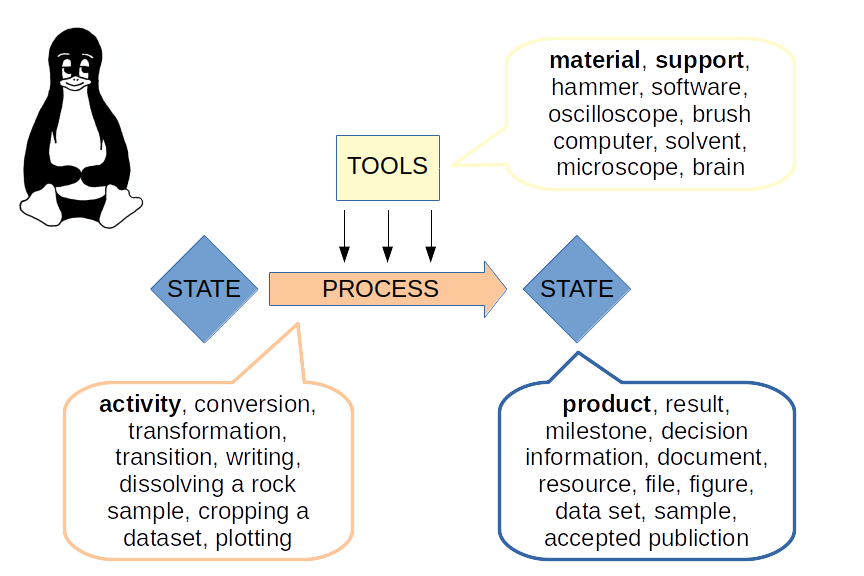
\includegraphics[height=4cm]{./images/box_workflow.png}

\column[c]{2.5cm}


%
\begin{beamerboxesrounded}[lower=gray,shadow=true]{
\footnotesize{
\textbf{Tools} \\
Material \\
support \\
\\
program function \\
Hammer \\
Software \\
Device \\
Computer \\
Solvent \\
Brain
}
}
\end{beamerboxesrounded}

\end{columns}
 



\end{frame}
%=============================================================================================
\begin{frame}{\insertsectionnumber{ |} Workflow - example}


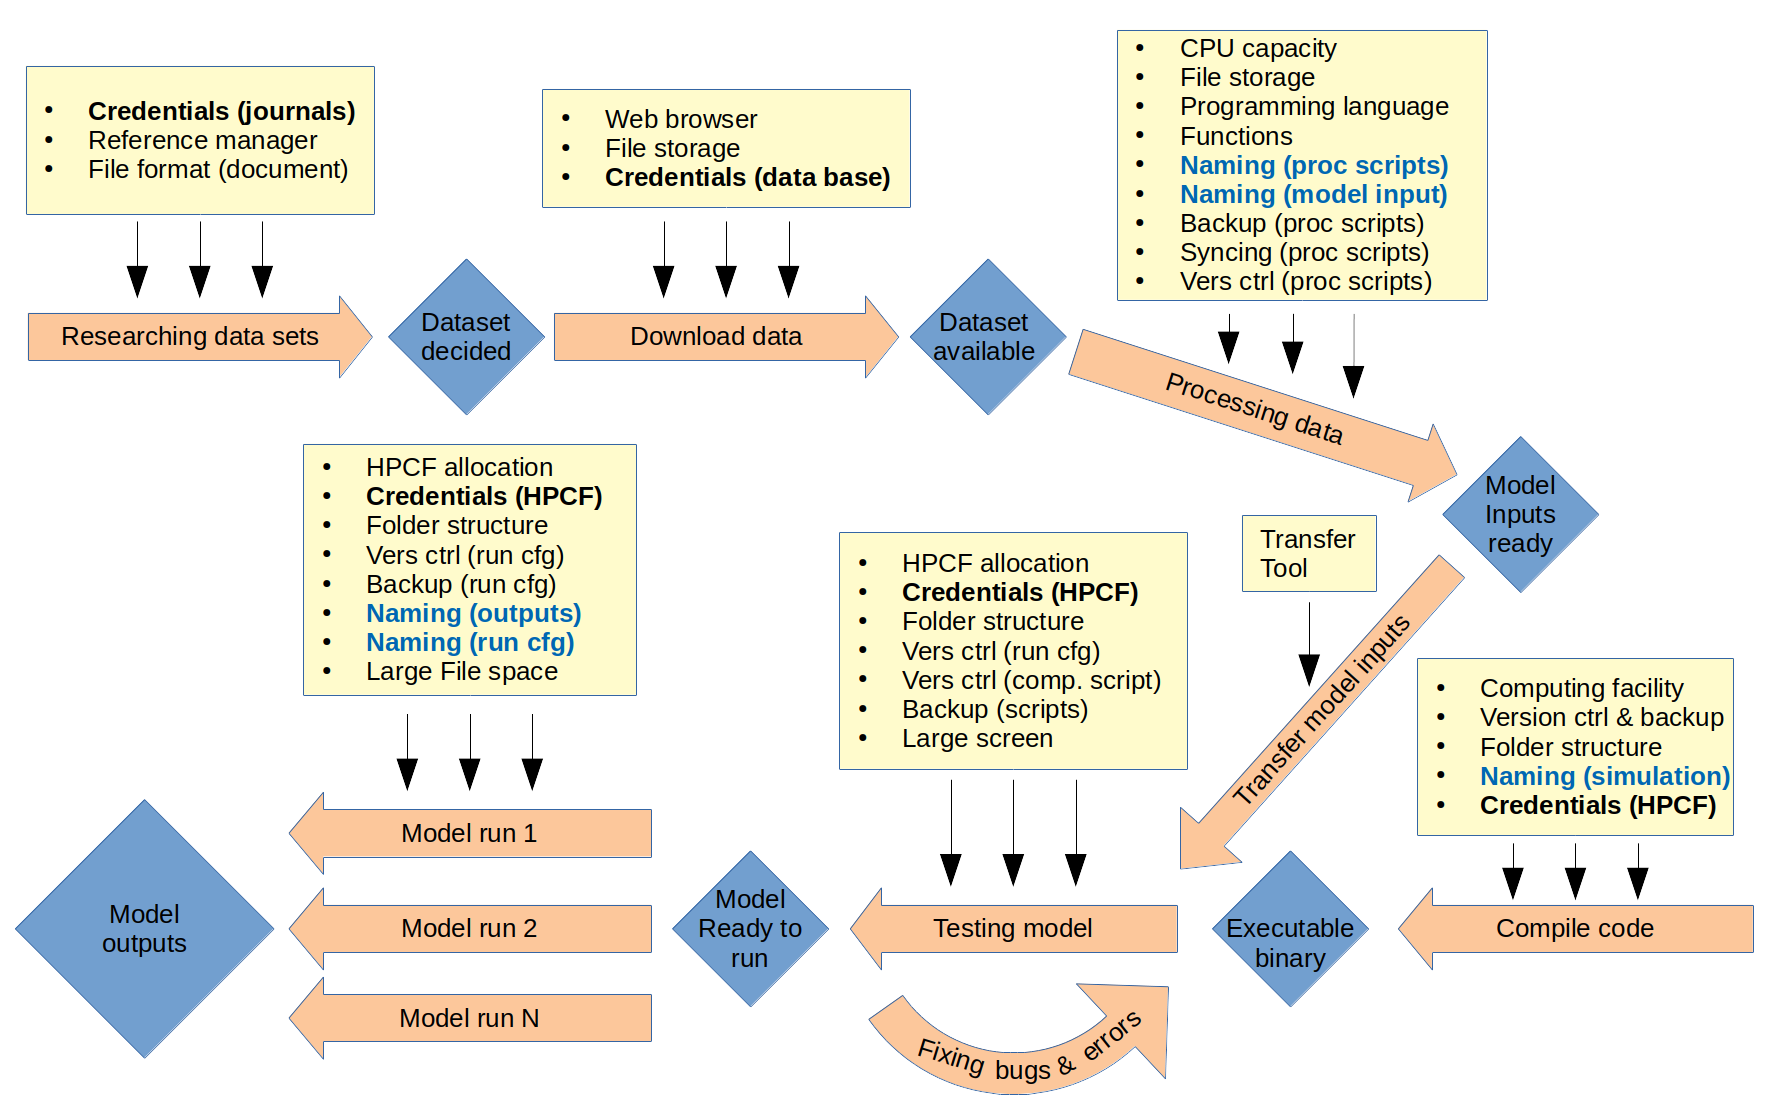
\includegraphics[width=11cm]{./images/workflow_example.png}

\begin{itemize}

\item Think of a small project in the recent past and sketch the associated workflow.
Examples could be: writing a Marsden one pager, set up and run a simulation or 
analyse rocks and record and store the data. Use the concept of State,  Process,  Tool

\end{itemize}

\end{frame}

%=============================================================================================

\begin{frame}{\insertsectionnumber{ |} Work Structure}

%\begin{beamerboxesrounded}[lower=gray,shadow=true]{
%\begin{itemize}
%\item What is a work structure? \\
\textit{A suitable \textbf{work structure} is a systematically organized work environment that \textbf{maps} one specific or a group of \textbf{workflows}.}
\begin{itemize}

\item The guiding principles to arrange the environment into a suitable structure are \\

\begin{itemize}
\item[\textbullet] Reproducability 
\item[\textbullet] Efficiency 
\item[\textbullet] Cost - in units of storage, processing time, computing load, money, FTE
\end{itemize}

\item For computer based environments the work structure typically consists of blocks such as 

\begin{itemize}
\begin{columns}

\column[c]{4cm}

\item[\textbullet] data sets
\item[\textbullet] software \& apps 
\item[\textbullet] compilers \& data language
\item[\textbullet] \textbf{file formats} 
\item[\textbullet] \textbf{version control}
\item[\textbullet] computer hardware 
\item[\textbullet] storage facilities
\column[c]{4cm}

\item[\textbullet] \textbf{backup procedure}
\item[\textbullet] communicaton model
\item[\textbullet] \textbf{folder structure}  
\item[\textbullet] exchange \& transfer protocol
\item[\textbullet] documentation
\item[\textbullet] \textbf{data handling}
\item[\textbullet] credential management


\end{columns}
\end{itemize}
\end{itemize}

%}
%\end{beamerboxesrounded}

\begin{itemize}
\item A specific work structure consists of a subset of these blocks. They are not absolute definitions and contain a deliberate degree of redundancy.
\item \textbf{The list of building blocks can be used as a stencil to filter out the important aspects in the workflow that need to be incorporated in your work structure.}
\vspace{0.2cm}
\item Find two entities that are important for your work structure and one that is negligible.  
\end{itemize}



\end{frame}

%=============================================================================================
%
\begin{frame}{\insertsectionnumber{ |} Work Structure - discussion}

\begin{itemize}
\item The implementation of a Work Structure can range from installing a plugin in your browser to manage all your online credentials to writing a large bash scripts that automatically synchronize all your Python scripts between your office desktop and your labotp at home.
\item Apart from the three guiding principles there are other motivations for a well organized work structure

\begin{itemize}
\item[\textbullet] the frustration having to recreate something that has been "lost" 
\item[\textbullet] can not afford to loose a good idea 
\item[\textbullet] wasting time to search for something
\end{itemize} 

\item Protect the products of your creativity, things that were made with your intellectual powers.
\item Even a costly computer model could be re-run. A good idea that you did not write down might not come back to you for any money. (How to create ideas is another lecture.)
\item There is no right or wrong work structure.  There is one or none.
\item \textbf{Feedback} - the process of tayloring your work structure around your own wokflow helps you streamlining the workflow itself.  

 %
\end{itemize}

\end{frame}

%=============================================================================================
%
\begin{frame}{\insertsectionnumber{ |} Folder Structure}

\begin{itemize}
\begin{columns}
\column[c]{6cm}
\item Arguably an effective folder structure is the most important and most visible component of a work structure.
\item There are multiple ways to sort / categorize files.
\begin{itemize}
\item[\textbullet] most commonly folders map the chronological order of tasks or task groups
\item[\textbullet] grouping by file types
\item[\textbullet] theme based 
\end{itemize} 
\item A good folder structure should
\begin{itemize}
\item[\textbullet] map the workflow
\item[\textbullet] contain no more than 6 to 10 subfolders for quick navigation
\item[\textbullet] have names that are self explaining
\item[\textbullet] separate data from tools
\item[\textbullet] separate backed up items from those that are not
\item[\textbullet] enables selective syncing with cloud services
\end{itemize} 




\item Design a future proof folder structure for your publications that matches your computer based workflow.
\column[c]{3cm}
\item Example modelling folder
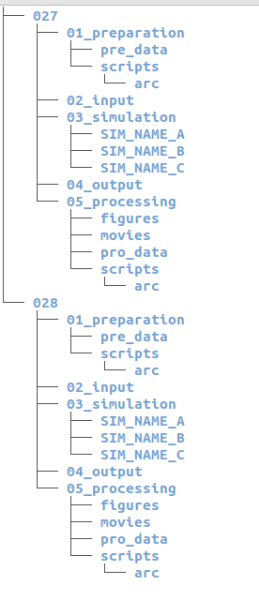
\includegraphics[height=7cm]{./images/folderstructure.png}
\end{columns}

\end{itemize}
 %

\end{frame}


%=============================================================================================
\begin{frame}{\insertsectionnumber{ |} Version Control - not a \textbf{How-To-Do} rather a \textbf{Do-NoMatter-How!}}
%The aim of this slide is not to show \textbf{How-To-Do} but to convey the message \textbf{Do-NoMatter-How!}
\begin{itemize}
\item There are many reasons why one has to go back to a previous version of something.
\item Do not ever delete or overwrite something that is a result of your intellectual powers (IP)
\item Freeing disk space is no longer a justified reason to delete. Even a 5000 line script consumes less than 200kB and available storage capacity is nowadays on the order of $10^6$ times bigger than that. 
%
\item One option is to use a Version Control System (VCS)
\begin{itemize}
\item[\textbullet] allows collaborators to work on the same project
\item[\textbullet] prevents overwriting of changes
\item[\textbullet] maintains a history of changes
\item[\textbullet] manages large repositories of files
\item[\textbullet] Distributed VCS are also a backup system
\end{itemize}
\item \textbf{Centralized VCS}
\begin{itemize}
\item[\textbullet] uses a central server for all files
\item[\textbullet] enables team collaboration
\item[\textbullet] vulnerable for single point of failure (disk of the central server)
\item[\textbullet] requires a separate backup workflow
\item[\textbullet] low risk of divergence
\end{itemize}
\item \textbf{Distributed VCS}
\begin{itemize}

\item[\textbullet] uses a central server and local clients
\item[\textbullet] clients mirror the full repository (implicitly failsafe)
\item[\textbullet] works offline
\item[\textbullet] risk of divergence is mitigated with sophisticated merging algorithms

\end{itemize}
\vspace{0.2cm}
\item What are you using for version control?
\end{itemize}

\end{frame}

%=============================================================================================
%\begin{frame}{\insertsectionnumber{ |} Version Control | git - repository \& init}
%\begin{itemize}
%\item Creating a repository  ...
%\end{itemize}
%\vspace{2cm}
%include in lecture ??? \\
%time factor ??
%\end{frame}
%%=============================================================================================
\begin{frame}{\insertsectionnumber{ |} Version Control | git - stage \& commit}

\begin{beamerboxesrounded}[lower=gray,shadow=true]{

clone the repository \\
\Verb+ git clone  https://github.com/sj-science//WinterSchool\_train\_repo +   \\
descend into project directory \\
\Verb+ cd /WinterSchool\_train\_repo +   \\
list the folder content, -l gives more information, -h makes the file size human readable \\
\Verb+ ls -lh  + 
}
\end{beamerboxesrounded}

\vspace{0.3cm}
\begin{itemize}

%\begin{beamerboxesrounded}[lower=gray,shadow=true]{
\item make a personal copy of the script, name it [your\_initials]\_script \\
%\Verb+ cp awesome...  your\_initials\_script + \\
\item execute the copied bash script  
%\Verb+ ./your\_initials\_script + 
%}
%\end{beamerboxesrounded}

\end{itemize}

\vspace{0.3cm}
\begin{beamerboxesrounded}[lower=gray,shadow=true]{

check the status of your local repository \\
\Verb+ git status +  \\
stage new file(s) for commit \\
\Verb+ git add your\_initials\_script  + \\
check status again \\
\Verb+ git status + \\
commiting the change to the local repository with a meaningful description \\
\Verb+ git commit -m 'adding a bash script that says "hello world"' + 
}
\end{beamerboxesrounded}

\end{frame}
%=============================================================================================
\begin{frame}{\insertsectionnumber{ |} Version Control | git - stage \& commit}


\begin{columns}
\column[c]{5cm}
\begin{beamerboxesrounded}[lower=gray,shadow=true]{
modify the file \\ % hand out vi cheat sheet
\Verb+ vi sj\_script + \\
new print message \\
\Verb+ echo "World says Hi" + \\
exit editor
\Verb+ Esc  :   x + 
}
\end{beamerboxesrounded}

\begin{beamerboxesrounded}[lower=gray,shadow=true]{
let's create another file  \\
\Verb+ touch empty\_file.txt + 
}
\end{beamerboxesrounded}

\column[c]{5cm}
\begin{beamerboxesrounded}[lower=gray,shadow=true]{
check status \\
\Verb+ git status + \\
- git lists new and modified files separately 
}
\end{beamerboxesrounded}

\begin{beamerboxesrounded}[lower=gray,shadow=true]{
\textit{stage} the modified file \\
\Verb+ git add sj\_script + \\
- only staged files can be commited to the repository
}
\end{beamerboxesrounded}

\end{columns}

\begin{beamerboxesrounded}[lower=gray,shadow=true]{
\textit{commit} the modification \& check status\\
\Verb+ git commit -m "changed the print out message" + \\
\Verb+ git status + \\ 
- unstaged changes are not effected by the commit
}
\end{beamerboxesrounded}


\vspace{1cm}
\begin{itemize}
%\begin{beamerboxesrounded}[lower=gray,shadow=true]{
\item modify the print script again, add a second line to the printed message \\
\item stage and commit the modified script and the new file to the repository
%\Verb+  +
%}
%\end{beamerboxesrounded}

\end{itemize}
\end{frame}


%=============================================================================================
\begin{frame}{\insertsectionnumber{ |} Version Control | git - display changes}
\begin{columns}

\column[c]{4cm}
\begin{beamerboxesrounded}[lower=gray,shadow=true]{
check status\\
\Verb+ git status + \\
display list of commits\\
\Verb+ git reflog + \\
display more details\\
\Verb+ git log + 
}
\end{beamerboxesrounded}

\column[c]{6cm}

\begin{beamerboxesrounded}[lower=gray,shadow=true]{
display the script \\
\Verb+ cat sj\_script + \\
display the script using git\\
\Verb+ git show [commitID1]:path/sj\_script +\\
display the script before the last commit \\
\Verb+ git show [commitID2]:path/sj\_script +
}
\end{beamerboxesrounded}
\end{columns}

\vspace{0.5cm}
%
\begin{beamerboxesrounded}[lower=gray,shadow=true]{
show difference in the script between two commits \\
\Verb+ git diff [commitID1]:path/sj\_script [commitID2]:path/sj\_script + \\
show all differences between two commits \\
\Verb+ git diff [commitID1] [commitID2] + 
}
\end{beamerboxesrounded}

\vspace{0.5cm}
\begin{itemize}
\item rename the file empty\_file.txt to [your\_initials]\_file.txt \\
\item edit the renamed file and add some text \\
\item stage and commit the change \\
\item display the differnce between your current (latest) and your first commit (hello world)
\end{itemize}

\end{frame}

%=============================================================================================
\begin{frame}{\insertsectionnumber{ |} Version Control | git - rollback}

\begin{beamerboxesrounded}[lower=gray,shadow=true]{
check status \\
\Verb+ git status + \\
show the commit history of the pointer \textit{HEAD} \\
\Verb+ git reflog +
}
\end{beamerboxesrounded}
\begin{columns}
\column[c]{5cm}

\begin{beamerboxesrounded}[lower=gray,shadow=true]{
soft rollback \\
\Verb+ git reset {-}{-}soft HEAD@\{[N]\} + \\
is equivalent to \\
\Verb+ git reset {-}{-}soft [commitID] + \\
changes are retained as staged \\
unstaged files are retained \\
\Verb+ git status+ \\
list files \\
\Verb+ ls -l + 
}
\end{beamerboxesrounded}


\column[c]{5cm}

\begin{beamerboxesrounded}[lower=gray,shadow=true]{
hard rollback \\
\Verb+ git reset {-}{-}hard [commitID]  + \\
changes are discarded \\
unstaged files are retained \\
\Verb+ git status+ \\
list files \\
\Verb+ ls -l +
}
\end{beamerboxesrounded}
\end{columns}


\begin{beamerboxesrounded}[lower=gray,shadow=true]{
check the pointer  \\
\Verb+ git reflog +
}
\end{beamerboxesrounded}


\vspace{0.5cm}
\begin{itemize}
\item move pointer \textit{HEAD} back to the most advanced commit
\end{itemize}


%\begin{itemize}
%\item create three files [your_initials]\_f1
%\end{itemize}


\end{frame}
%=============================================================================================
\begin{frame}{\insertsectionnumber{ |} Version Control | git - push \& pull}

\begin{beamerboxesrounded}[lower=gray,shadow=true]{
check status \\
\Verb+ git status + \\
\Verb+ Your branch is ahead of 'origin/play\_branch\_sj' by 3 commits. + \\
\Verb+   (use "git push" to publish your local commits) + \\
says we can fast forward with a simple command - GREAT! 
}
\end{beamerboxesrounded}

\begin{beamerboxesrounded}[lower=gray,shadow=true]{
push changes to the online repository \\

\Verb+ git push + \\
\footnotesize{
\Verb+ +\\
\Verb+ To https://github.com/golledni//WinterSchool\_train\_repo + \\
\Verb+ ! [rejected]        play\_branch\_sj -> play\_branch\_sj (fetch first) + \\
\Verb+ error: failed to push some refs to 'https://github.com/golledni//WinterSchool\_train\_repo' + \\
\Verb+ hint: Updates were rejected because the remote contains work that you do + \\
\Verb+ hint: not have locally. This is usually caused by another repository pushing + \\
\Verb+ hint: to the same ref. You may want to first integrate the remote changes + \\
\Verb+ hint: (e.g., 'git pull ...') before pushing again. + \\
\Verb+ hint: See the 'Note about fast-forwards' in 'git push {-}{-}help' for details. +}
}
\end{beamerboxesrounded}
\begin{itemize}
\item there is no such thing as "simultaneous" work on a central project / repository / document
\item modifications need to be applied sequentially to avoid divergence 
\item even google.docs commits changes from collaborators sequentially - but very fast 
\end{itemize}

\end{frame}

%=============================================================================================
\begin{frame}{\insertsectionnumber{ |} Version Control | git - merge}
\begin{itemize}
\item Two choices - merge or new branch ...
\item merge \\

\Verb+git pull + \\
\footnotesize{
\Verb+ + \\
\Verb+  GNU nano 2.9.3                  /home/..../.git/MERGE\_MSG + \\
\Verb+Merge branch 'main' of https://github.com/sj-science//WinterSchool\_train\_repo into main +\\
\Verb+ + \\
\Verb+\# Please enter a commit message to explain why this merge is necessary, +\\
\Verb+\# especially if it merges an updated upstream into a topic branch. +\\
\Verb+\# +\\
\Verb+\# Lines starting with '\#' will be ignored, and an empty message aborts +\\
\Verb+\# the commit. + 
}
\end{itemize}
\begin{itemize}


\item the merging happens on the local repository \\
\Verb+ ls + \\
\item remote change has been pulled to local folder
\item the file you originall committed has been uncomitted \\

\Verb+git status + \\

\footnotesize{
\Verb+ +\\
\Verb+On branch main +\\
\Verb+Your branch and 'origin/main' have diverged, +\\
\Verb+and have 1 and 2 different commits each, respectively. +\\
\Verb+  (use "git pull" to merge the remote branch into yours) +\\

\Verb+All conflicts fixed but you are still merging. +\\
\Verb+  (use "git commit" to conclude merge) +\\

\Verb+Changes to be committed: +\\
\Verb+new file:   blub.txt +\\
}
\end{itemize}
\end{frame}
%=============================================================================================
\begin{frame}{\insertsectionnumber{ |} Version Control | git - merge}
\begin{itemize}


\item re-commit your new file \\
\end{itemize}
\Verb+git commit -m "re-commit my new file to finish merge" +\\
\Verb+git status +\\

\begin{tcolorbox}[width=11cm,
    fontupper=\normalsize,drop fuzzy shadow southwest,
    boxrule=0.4pt,sharp corners,colframe=yellow!80!black,colback=yellow!10]
\footnotesize{
\Verb+On branch main +\\
\Verb+Your branch is ahead of 'origin/main' by 2 commits. +\\
\Verb+  (use "git push" to publish your local commits)  +\\
\Verb+  +\\
\Verb+nothing to commit, working tree clean  +
}
\end{tcolorbox}

\normalsize{
\Verb+git push +\\
\Verb+git status +\\
}

\begin{tcolorbox}[width=11cm,
    fontupper=\normalsize,drop fuzzy shadow southwest,
    boxrule=0.4pt,sharp corners,colframe=yellow!80!black,colback=yellow!10]
\footnotesize{
\Verb+On branch main +\\
\Verb+Your branch is up to date with 'origin/main'. +\\
\Verb+ +\\
\Verb+nothing to commit, working tree clean +

}
\end{tcolorbox}


%\tcbox[enhanced,fontupper=\large\bfseries,drop fuzzy shadow southwest,
%    boxrule=0.4pt,sharp corners,colframe=yellow!80!black,
%    colback=yellow!10]{(G) text write here}


\end{frame}
%=============================================================================================
\begin{frame}{\insertsectionnumber{ |} Version Control | git - branch}

\Verb+ git push + \\
\begin{tcolorbox}[width=11cm,
    fontupper=\normalsize,drop fuzzy shadow southwest,
    boxrule=0.4pt,sharp corners,colframe=yellow!80!black,colback=yellow!10]    
\footnotesize{
\Verb+ To https://github.com/sj-science//WinterSchool\_train\_repo + \\
\Verb+ ! [rejected]        play\_branch\_sj -> play\_branch\_sj (fetch first) + \\
\Verb+ error: failed to push some refs to 'https://github.com/sj-science//WinterSchool\_train\_repo' + \\
\Verb+ hint: Updates were rejected because the remote contains work that you do + \\
\Verb+ hint: not have locally. This is usually caused by another repository pushing + \\
\Verb+ hint: to the same ref. You may want to first integrate the remote changes + \\
\Verb+ hint: (e.g., 'git pull ...') before pushing again. + \\
\Verb+ hint: See the 'Note about fast-forwards' in 'git push {-}{-}help' for details. +}
\end{tcolorbox}


\Verb+git branch + \\
\begin{tcolorbox}[width=11cm,
    fontupper=\normalsize,drop fuzzy shadow southwest,
    boxrule=0.4pt,sharp corners,colframe=yellow!80!black,colback=yellow!10]
\footnotesize{
\Verb+  main + 
}
\end{tcolorbox}
\begin{itemize}
\item create a new branch
\end{itemize}
\Verb+git checkout -b sj\_branch +\\
\begin{tcolorbox}[width=11cm,
    fontupper=\normalsize,drop fuzzy shadow southwest,
    boxrule=0.4pt,sharp corners,colframe=yellow!80!black,colback=yellow!10]
\footnotesize{
\Verb+Switched to a new branch 'sj\_branch' +
}
\end{tcolorbox}


\Verb+git branch + \\
\begin{tcolorbox}[width=11cm,
    fontupper=\normalsize,drop fuzzy shadow southwest,
    boxrule=0.2pt,sharp corners,colframe=yellow!80!black,colback=yellow!10]
\footnotesize{
\Verb+ main + \\
\Verb+$*$sj\_branch +
}
\end{tcolorbox}

\end{frame}
%=============================================================================================
\begin{frame}{\insertsectionnumber{ |} Version Control | git - branch}


\begin{itemize}
\item check new branch
\end{itemize}

\Verb+git status; echo; ls +\\
\begin{tcolorbox}[width=11cm,
    fontupper=\normalsize,drop fuzzy shadow southwest,
    boxrule=0.4pt,sharp corners,colframe=yellow!80!black,colback=yellow!10]
\footnotesize{
\Verb+On branch sj\_branch + \\
\Verb+nothing to commit, working tree clean + \\
\Verb+ +\\
\Verb+sj\_script.txt +
}
\end{tcolorbox}

%
%\Verb+ls +\\
%\begin{tcolorbox}[width=11cm,
%    fontupper=\normalsize,drop fuzzy shadow southwest,
%    boxrule=0.4pt,sharp corners,colframe=yellow!80!black,colback=yellow!10]
%\footnotesize{
%\Verb+ sj\_script.txt + 
%}
%\end{tcolorbox}


\begin{itemize}
\item add the new branch to the remote repository
\end{itemize}

\Verb+ git push -u origin sj\_branch + \\
\begin{tcolorbox}[width=11cm,
    fontupper=\normalsize,drop fuzzy shadow southwest,
    boxrule=0.4pt,sharp corners,colframe=yellow!80!black,colback=yellow!10]
\footnotesize{
\Verb+branch + \\
\Verb+Counting objects: 12, done.+ \\
\Verb+Delta compression using up to 8 threads.+ \\
\Verb+Compressing objects: 100\% (9/9), done.+ \\
\Verb+Writing objects: 100\% (12/12), 1.40 KiB | 1.40 MiB/s, done.+ \\
\Verb+Total 12 (delta 3), reused 0 (delta 0)+ \\
\Verb+remote: Resolving deltas: 100\% (3/3), done.+ \\
\Verb+remote: + \\
\Verb+remote: Create a pull request for 'sj\_branch' on GitHub by visiting:+ \\
\Verb+remote:      https://github.com/sj-science/WinterSchool\_train\_repo/pull/new/sj\_branch+ \\
\Verb+remote: + \\
\Verb+To https://github.com/sj-science/WinterSchool\_train\_repo.git+ \\
\Verb+ $*$ [new branch]      sj\_branch -> sj\_branch+ \\
\Verb+Branch 'sj\_branch' set up to track remote branch 'sj\_branch' from 'origin'.+ 
}
\end{tcolorbox}

\end{frame}
%=============================================================================================
\begin{frame}{\insertsectionnumber{ |} Version Control | git - branch}


\Verb+git status +\\
\begin{tcolorbox}[width=11cm,
    fontupper=\normalsize,drop fuzzy shadow southwest,
    boxrule=0.4pt,sharp corners,colframe=yellow!80!black,colback=yellow!10]
\footnotesize{
\Verb+On branch sj\_branch +\\
\Verb+Your branch is up to date with 'origin/sj\_branch'. +\\
\Verb+ +\\
\Verb+nothing to commit, working tree clean +
}
\end{tcolorbox}

\begin{itemize}
\item your colleague can now see and access (checkout) your new branch
\end{itemize}

\Verb+git fetch +\\
\begin{tcolorbox}[width=11cm,
    fontupper=\normalsize,drop fuzzy shadow southwest,
    boxrule=0.4pt,sharp corners,colframe=yellow!80!black,colback=yellow!10]
\footnotesize{
\Verb+remote: Enumerating objects: 3, done. +\\
\Verb+remote: Counting objects: 100\% (3/3), done. +\\
\Verb+remote: Compressing objects: 100\% (2/2), done. +\\
\Verb+remote: Total 2 (delta 1), reused 1 (delta 0), pack-reused 0 +\\
\Verb+Unpacking objects: 100\% (2/2), done. +\\
\Verb+From https://github.com/sj-science/WinterSchool\_train\_repo +\\
\Verb+ $*$ [new branch]      sj\_branch  -> origin/sj\_branch +
}
\end{tcolorbox}

\Verb+git branch -r +\\
\begin{tcolorbox}[width=11cm,
    fontupper=\normalsize,drop fuzzy shadow southwest,
    boxrule=0.4pt,sharp corners,colframe=yellow!80!black,colback=yellow!10]
\footnotesize{
\Verb+origin/HEAD -> origin/main +\\
\Verb+origin/main +\\
\Verb+origin/sj\_branch +
\Verb+ +
}
\end{tcolorbox}

\end{frame}
%=============================================================================================
\begin{frame}{\insertsectionnumber{ |} Version Control | git checkout}

\Verb+git checkout sj\_branch +\\
\begin{tcolorbox}[width=11cm,
    fontupper=\normalsize,drop fuzzy shadow southwest,
    boxrule=0.4pt,sharp corners,colframe=yellow!80!black,colback=yellow!10]
\footnotesize{
\Verb+sj\_branch +\\
\Verb+Switched to branch 'sj\_branch' +\\
\Verb+Your branch is up to date with 'origin/sj\_branch'.  + 
}
\end{tcolorbox}
%
\vspace{1cm}

\begin{itemize}
\item Create and switch to your own branch "your\_initials\_branch"
\item Create another bash script with a message to your colleagues.
\item Commit this file to the new branch
\item Push the branch to track its remote counterpart
\item Checkout one of your colleagues new branches and find out their message to you.
\end{itemize}

\end{frame}
%=============================================================================================
\begin{frame}{\insertsectionnumber{ |} Version Control | Alternatives}
\begin{itemize}
\item \textbf{git} follows a distribution model where users maintain a local copy \\
its main strength is its easy branching and merging capability 
\item hosting providers for git repositories \textbf{GitHub, GitLab, azure, Bitbucket} and others 

\item \textbf{svn} is a git alternative that follows a centralized model
\item using git as a simple backup tool is slightly overkill considering its powerful features
 \\
\item \textbf{onedrive} is a commercial cloud service (1TB included in VUW and NIWA accounts) \\
\begin{itemize}
\item[\textbullet] automatically creates an instant \textit{commit}+\textit{push} everytime a document is saved locally\
\item[\textbullet] version history can be accessed via Office-365 
\item[\textbullet] native client in MS-Win, clients available for Android, MacOS and Linux  
\end{itemize}
\item \textbf{seafile} is an opensource file sync{\&}share engine (\url{www.seafile.com}) 
\begin{itemize}
\item[\textbullet] comparable to onedrive seafile syncs instantly any changes with an online repository 
\item[\textbullet] works with command line \& gui across all plattforms 
\item[\textbullet] SGEES offers 20GB server space through using seafile (talk to Aleks Beliaev) 
\end{itemize}
\end{itemize}

\begin{columns}
\column[c]{7.5cm}

\begin{itemize}
\item \textbf{alternatives} 
\begin{itemize}
\item[\textbullet] \textbf{Google Drive}, \textbf{MEGAsync}, \textbf{Amazon Cloud Drive}
\item[\textbullet] many email providers offer a cloud service 
\item[\textbullet] the trick is to find a client app that works for your OS
\item[\textbullet] \textbf{rsync} \&  external harddrive
\item[\textbullet] \textbf{overleaf} for tex documents
\end{itemize} 
\item How about naming files in a suitable fashion?


\end{itemize}
\column[c]{2cm}

\includegraphics[height=2.0cm]{./images/twinky.jpg}
\end{columns}
\end{frame}

%%=============================================================================================
%
\begin{frame}{\insertsectionnumber{ |} File Naming}
\begin{itemize}
\item Establishing a good naming convention 
\begin{itemize}
\item[\textbullet] helps to maintain structure inside folders
\item[\textbullet] is the simplest method of version management \& control
\item[\textbullet] avoids duplicities
\item[\textbullet] helps manually syncing folders
\item[\textbullet] helps avoiding long names
\end{itemize}
%  
\item A good file name file\_name.apx
\begin{itemize}
\item[\textbullet] contains all valid information to clearly identify the file content
\item[\textbullet] should be no longer than 12 letters
\item[\textbullet] does \textbf{NOT} contain spaces
\item[\textbullet] leaves the file extension as is
\end{itemize}
\item example \\
023\_bry\_ACOSM\_9km24\_V02.nc \\
article\_draft\_v12\_sj1.docx \\
RSSM\_84Bg2bT3\_4avg\_abs\_2118\_fig1\_Dec\_Jan\_966.png \\
\end{itemize}
%
%\vspace{2cm}
\end{frame}

%%=============================================================================================

\begin{frame}{\insertsectionnumber{ |} Data Handling - Access \& Backup}
\begin{itemize}
\item \textbf{Storing and access of large data files}
\item Load only what you need (crop and slicing of data).
\item Make sure filesystems are mounted sufficiently "close" to the processing instance.
\begin{itemize}

\item[\textbullet] Loading 1GB from a mounted network drive can test your patience
\item[\textbullet] Sufficient USB3 link is now standard for portable drives  

\end{itemize}
\item Portable and therefore local drives are fine until processing becomes too demanding for the labtop
\item Avoid duplicate copies
\item Establish a universal mount point for data storage in your folder structure 
\begin{itemize}

\item[\textbullet] avoids the need for hard coding (changing) access paths in processing scripts

\end{itemize}
\vspace{0.2cm}
\item \textbf{Backup strategy for data and model outputs} \\
Depends on size and cost of reproducing. 
\item Collected Field data 
\begin{itemize}
\item[\textbullet] Virtually not reproducible, unless you get another Marsden to revisit your field site
\item[\textbullet] Needs fail save backup e.g. redundancy. Lab repository + Cloud Service + external disk. 
\end{itemize}
\item Model outputs from your own simulations.
\begin{itemize}
\item[\textbullet] Too big for redundant backups.
\item[\textbullet] In case of disaster they can be reproduced by rerunning the model although there is a cost (only if a complete backup of the runtime script and input conditions exists!)
\end{itemize}
\item Downloaded Data
\begin{itemize}
\item[\textbullet] If the repository (like CMIP database) is unlikely to be decommissioned no need for backup.
\end{itemize}

\end{itemize}



\end{frame}

%%=============================================================================================

\begin{frame}{\insertsectionnumber{ |} Best Practise}


\includegraphics[width=12.0cm]{./images/bestpractise.png}

%Know when to stop quick-and-dirty and start flash and clean. \\
%Start folder names with a number. (fixed order everywhere) \\
%Auto sync folder folders across all multiple platforms. \\
%use cloud services selectively \\
%stay within your OS. do not edit things on windows and then copy back \\
%there is always Ctrl+F,  cat * | grep 'figurexyz'
%
%good example "write a Marsden one pager", my challenge will be: in 5 years time you remember a certain piece of information from that project i.e. a comment Nick made on an early version of the proposal.
%think about the document format word vs latex \\
%ftp server at VUW from aleks \\
%
%good naming convention \\
%do not use spaces in file or folder names!!! \\
%space introduces ambiguity\\
%dont mix backup systems\\
%
%synchronizing between machines (desktop at work, desktop at home, labtop and super computer)
%rsync

\end{frame}
%%%%%%%%%%%%%%%%%%%%%%%%
%

%%%%%%%%%%%%%%%%%%%%%%%% END CONTENT %%%%%%%%%%%%%%%%%%%%%%
